\chapter{Ergebnisse}
\label{ch:chapter05}

\section{Einleitung und Datenaufbereitung}
In diesem Kapitel werden die Ergebnisse der Performance-Messungen präsentiert. Da sehr viele Daten vorliegen, werden die wichtigsten 
Erkentnisse in zusammengefasster Form dargestellt. Alle Rohdaten und detaillierten Analysen sind im Anhang zu finden und werden an den 
entsprechenden Stellen in diesem Kapitel referenziert.

\section{Statistische Signifikanz}
\paragraph[short]{Hypothesentests H1}
Die Performance-Veränderungen durch die Instrumentierung der Funktionen mit OpenTelemetry haben sich anhand der 
Bootstrap-Konfidenzintervalle, für alle Metriken und Benchmarks als statistisch signifikant erwiesen, da keines 
der der Intervalle die Null einschließt (siehe Anhang~\ref{app:boot:cold}).

\paragraph[short]{Hypothesentests H2}
Die Unterschiede im Performance-Overhead zwischen allen 3 Sprachen für alle Benchmarks und Metriken wurden ebenfalls als 
statistisch signifikant bestätigt, da alle p-Werte unter dem korrigierten Signifikanzniveau von 
\(\alpha_{\text{korrekt}} = 0{,}00067\) liegen (siehe Anhang~\ref{boot:res:cold} und~\ref{boot:res:hot}).

\section{Absolute Messwerte und relativer Overhead (Median)}
Aufgrund der Vielzahl der Ergebnisse (jeweils 75 Kombinationen aus 
3 Sprachen, 5 Benchmarks, 3 Metriken und 2 Starttypen), werden die Ergebnisse anhand von Ranglisten präsentiert. Die Ranglisten 
wurden in Form von Tabellen, separat für mediane absolute Messwerte ohne OTel, mit OTel und Overhead basierend auf sowohl den 
Originaldaten als auch den Bootstrap-Resamples erstellt. 
Die Tabellen zeigen, 
wie häufig jede Sprache bei den fünf Benchmarks den ersten, zweiten oder dritten Platz belegt hat (aufgeschlüsselt nach 
Metriken) für Kalt- und Warmstarts. Der kleinste mediane absolute Messwert (in MB oder ms) oder Overhead (in \%) erhält den ersten Platz. 

\subsection{Mediane Overheads}
Die Ranglisten der relativen Overheads sind auf Basis der Originaldaten und der Bootstrap-Resamples nicht identisch 
(siehe Anhang~\ref{app:rankings}). Das liegt an den unterschiedlichen Mengengrößen der Overhead-Mediane (1 Originalmedian vs. 
100.000 Bootstrap-Mediane pro Metrik). Daher werden hier nur die Bootstrap-Ranglisten präsentiert, da sie eine bessere statistische 
Aussagekraft besitzen.
\begin{table}[H]
\centering
\footnotesize
\setlength{\tabcolsep}{8pt}
\caption{Rangliste prozentualer Overhead}
\label{app:ranking-overhead-cold-bootstrap}
\begin{tabular}{|l|c|}
\hline
\textbf{Metrik} & \textbf{Platz (1./2./3.)} \\
\hline
& \textbf{Kaltstarts} \\
\hline
Init Duration & Java: 2/3/0, Node.js: 0/0/5, Python: 3/2/0 \\
\hline
Duration      & Java: 0/3/2, Node.js: 2/0/3, Python: 3/2/0 \\
\hline
Max Memory    & Java: 2/3/0, Node.js: 0/0/5, Python: 3/2/0 \\
\hline
Kombiniert (15) & Java: 4/9/2, Node.js: 2/0/13, Python: 9/6/0 \\
\hline
& \textbf{Warmstarts} \\
\hline
Duration      & Java: 3/2/0, Node.js: 2/0/3, Python: 0/3/2 \\
\hline
Max Memory    & Java: 1/4/0, Node.js: 1/1/3, Python: 3/0/2 \\
\hline
Kombiniert (10) & Java: 4/6/0, Node.js: 3/1/6, Python: 3/3/4 \\
\hline
& \textbf{Kalt \& Warm} \\
\hline
Gesamt (25)   & Java: 8/15/2, Node.js: 5/1/19, Python: 12/9/4 \\
\hline
\end{tabular}
\end{table}

\subsection{Mediane Absolute Messwerte} 
Die Ranglisten der absoluten Messwerte der instrumentierten und nicht-instrumentierten 
Funktionen sind identisch auf Basis der Originaldaten und der Bootstrap-Resamples, was die Stabilität der Ergebnisse unterstreicht 
(siehe Anhang~\ref{app:rankings}). 
Es werden hier nur die Ranglisten der instrumentierten Funktionen präsentiert, da nur sie praxisrelevant sind.

\begin{table}[H]
\centering
\footnotesize
\setlength{\tabcolsep}{8pt}
\caption{Rangliste absolute Werte mit OTel}
\label{app:ranking-with-otel}
\begin{tabular}{|l|c|}
\hline
\textbf{Metrik} & \textbf{Platz (1./2./3.)} \\
\hline
& \textbf{Kaltstarts} \\
\hline
Init Duration & Java: 0/0/5, Node.js: 0/5/0, Python: 5/0/0 \\
\hline
Duration & Java: 0/0/5, Node.js: 0/5/0, Python: 5/0/0 \\
\hline
Max Memory & Java: 0/0/5, Node.js: 0/5/0, Python: 5/0/0 \\
\hline
Kombiniert (15) & Java: 0/0/15, Node.js: 0/15/0, Python: 15/0/0 \\
\hline
& \textbf{Warmstarts} \\
\hline
Duration & Java: 1/1/3, Node.js: 0/4/1, Python: 4/0/1 \\
\hline
Max Memory & Java: 0/0/5, Node.js: 0/5/0, Python: 5/0/0 \\
\hline
Kombiniert (10) & Java: 1/1/8, Node.js: 0/9/1, Python: 9/0/1 \\
\hline
& \textbf{Kalt \& Warm} \\
\hline
Gesamt (25) & Java: 1/1/23, Node.js: 0/24/1, Python: 24/0/1 \\
\hline
\end{tabular}
\end{table}

\section{Sprachspezifische Unterschiede}
Kaltstarts

Duration (mit OTel, Median): größter Unterschied bei dynamodb-write, 1800,79 ms (Java 1849,57 vs Python 48,78).
Duration (Overhead): größter Unterschied bei get-request, 245,54 Prozentpunkte (Java 220,70 \% vs Node.js -24,84 \%).
Init Duration (mit OTel, Median): größter Unterschied bei dynamodb-write, 3129,38 ms (Java 4350,58 vs Python 1221,20).
Init Duration (Overhead): größter Unterschied bei post-request, 520,70 Prozentpunkte (Node.js 805,21 \% vs Java 284,51 \%).
Max Memory Used (mit OTel, Median): größter Unterschied bei invoke, 142,00 MB (Java 250,00 vs Python 108,00).
Max Memory Used (Overhead): größter Unterschied bei dynamodb-write, 43,39 Prozentpunkte (Node.js 66,99 \% vs Python 23,60 \%).

Warmstarts

Duration (mit OTel, Median): größter Unterschied bei invoke, 14,73 ms (Python 31,24 vs Java 16,51).
Duration (Overhead): größter Unterschied bei get-request, 27,19 Prozentpunkte (Python 44,96 \% vs Node.js 17,77 \%).
Init Duration (mit OTel, Median): keine Warmstart-Daten vorhanden.
Init Duration (Overhead): keine Warmstart-Daten vorhanden.
Max Memory Used (mit OTel, Median): größter Unterschied bei invoke, 141,00 MB (Java 250,00 vs Python 109,00).
Max Memory Used (Overhead): größter Unterschied bei dynamodb-write, 38,66 Prozentpunkte (Node.js 62,26 \% vs Python 23,60 \%).

\section{Kostenabschätzung für die instrumentierten Funktionen}
Die Kosten für die instrumentierten Funktionen wurden auf Basis der Bootstrap-Mediane der 
absoluten Messwerte mithilfe der in~\ref{sec:kostenmodell} beschriebenen Formel berechnet. 
\begin{figure}[H]
\centering
\caption{Günstigste Varianten der 5 Microbenchmarks für 1 Million Anfragen.}
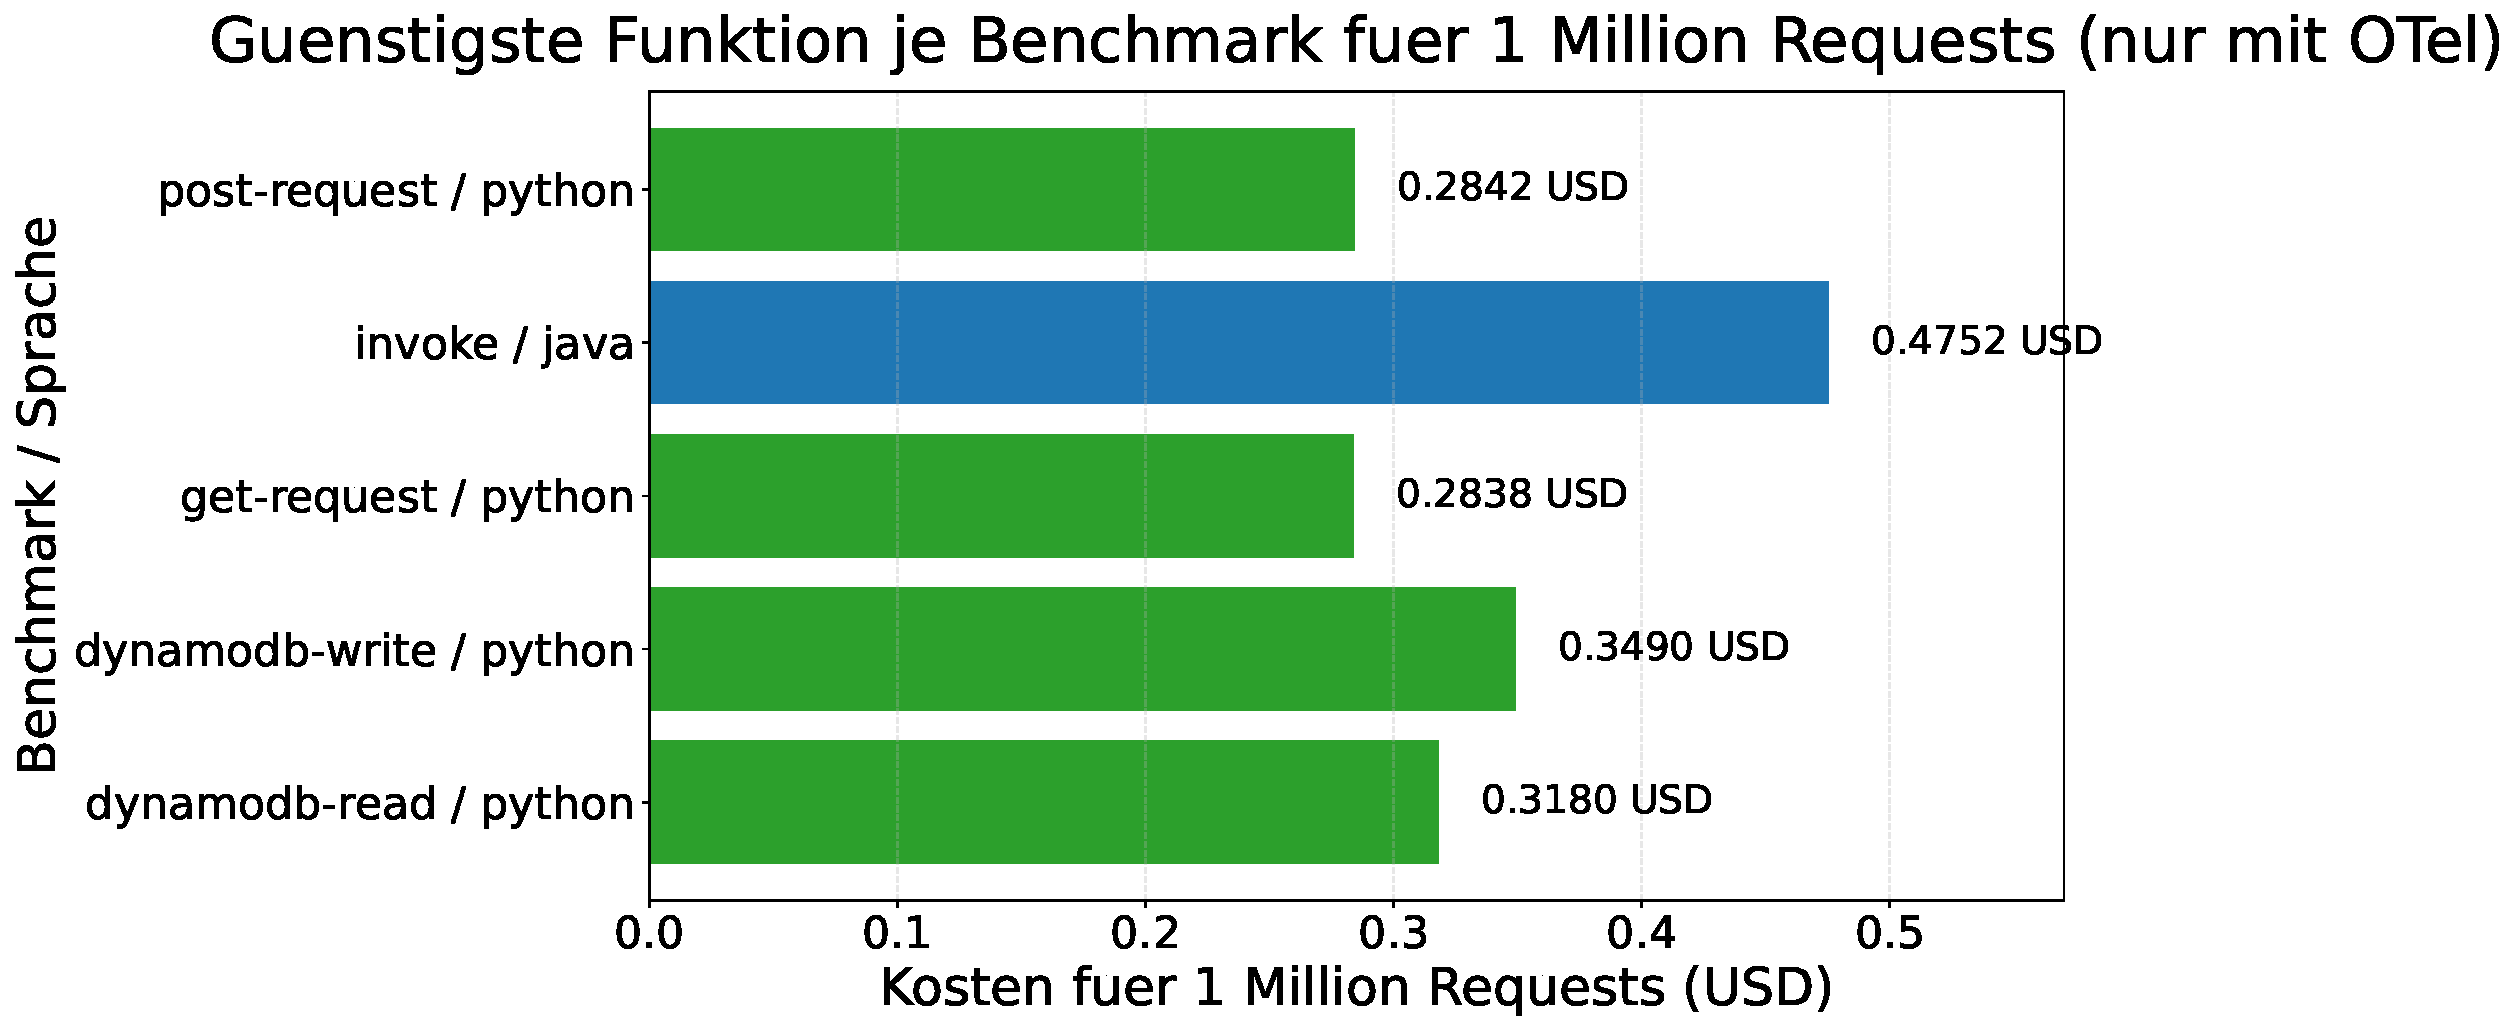
\includegraphics[width=1\textwidth]{gfx/examples/lambda_cost_1m_requests_otel_cheapest_per_benchmark_bar.pdf}
\end{figure}